\section*{Занятие 8}
\begin{exercise}[1]
	$Y=(X-1)^2$
	\begin{itemize}
		\item $X=-1 \Rightarrow Y=4$
		\item $X=0 \Rightarrow Y=1$
		\item $X=2 \Rightarrow Y=1$
		\item $X=3 \Rightarrow Y=4$
	\end{itemize}
	$\Rightarrow P(Y=1) = P(X=0)+P(X=2)=0,4+0,3=0,7$ \\ $P(Y=4) = P(X=-1) + P(X=3)=0,1+0,2=0,3$
	Мы получим закон распределения
	\begin{center}
		\begin{tabular}{|c|c|c|}
			\hline
			$Y$ & 1 & 4 \\ \hline
			$P$ & 0,7 & 0,3 \\ \hline
		\end{tabular}
	\end{center}
\end{exercise}

\begin{exercise}[2]
	$f(x) = \frac{1}{b-a}$, $0 < a \leq x \leq b$ и $Y=X^2$ \\ $\Rightarrow x=\sqrt{y}$, $a^2 \leq y \leq b^2$ \\ Плотность вероятности случайной величины $Y$:
	
	$g(y) = \frac{1}{b-a} \cdot \Big|(\sqrt{y})'\Big| = \frac{1}{2(b-a)\cdot \sqrt{y}}$, $a^2 \leq y \leq b^2$
\end{exercise}

\begin{exercise}[3]
	$f(x) = \frac{x}{\sigma^2} \exp{-\frac{x^2}{2\sigma^2}}$, $x \geq 0$ и $Y=\sigma/X$ \\ $\Rightarrow x=\sigma/y$ и $y > 0$. Поэтому плотность распределения случайной величины $Y$:
	
	$g(y) = \frac{\sigma}{y\sigma^2} \exp\Big(-\frac{\sigma^2}{y^2 \cdot 2 \sigma^2}\Big) \Big|\Big(\frac{\sigma}{y}\Big)'\Big| = \frac{1}{y \sigma} \exp\Big(-\frac{1}{2y^2}\Big) \cdot \frac{\sigma}{y^2} = y^{-3} \exp\Big(-\frac{1}{2y^2}\Big)$
\end{exercise}

\begin{exercise}[4] Мы обозначим через $X$ угол между осью абсцисс и направлением из начала координат на точку касания. Мы получим длину от точки касания до точки ее пересечения с осью $Ox$: $H=AC=\tg X$, $x \in [0, \pi/2]$
	\begin{figure}[h]
	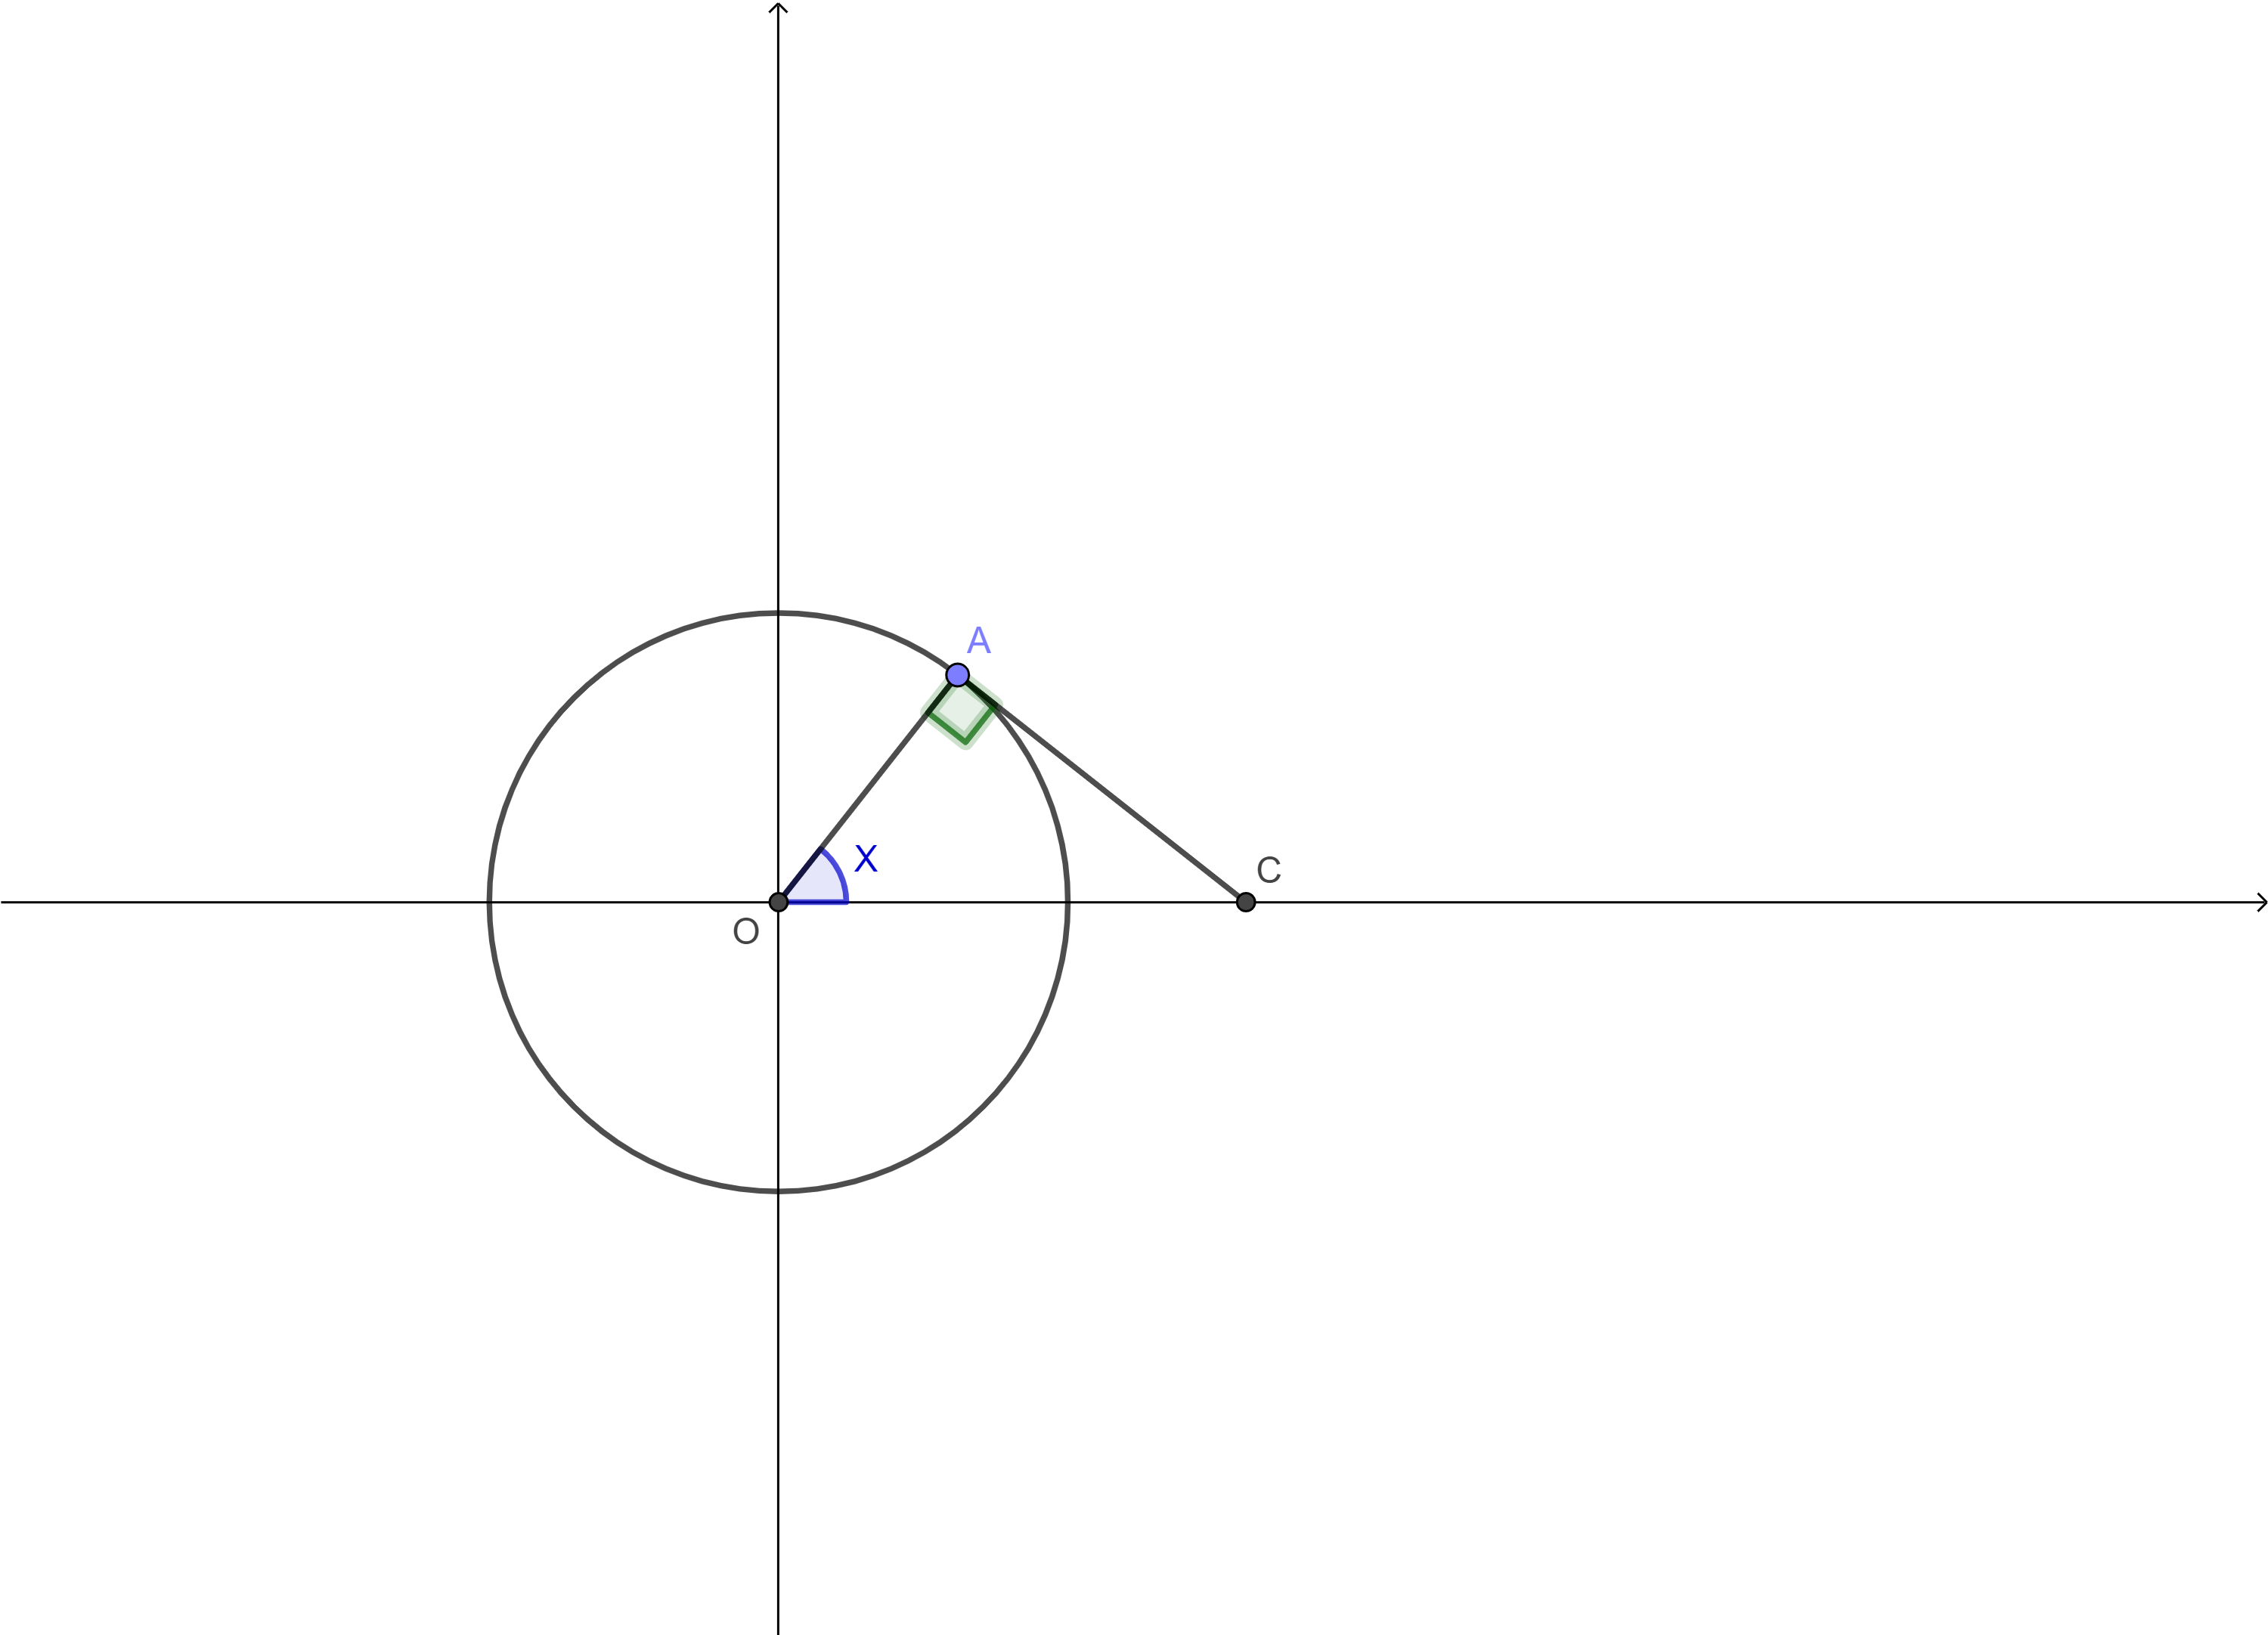
\includegraphics{exercise4-8.png}
	\centering
	\end{figure}

У нас есть $H=\tg X$, $x \in [0, \pi/2]$. Следовательно, $X$ имеет равномерное на $[0, \pi/2]$ распределения с функцией плотности вероятности $f(x)=\frac{2}{\pi}$. Поэтому $x = \arctg h$, $h \geq 0$

Мы получим $g(h)=\frac{2}{\pi} \cdot \Big|(\arctg h)'\Big| = \frac{2}{\pi \sqrt{1+h^2}}$, $h > 0$

При $h \leq 0$, $$F(h) = \int_{-\infty}^{h}0\,dh = 0$$

При $h > 0$, $$F(h) = \int_{-\infty}^{h}g(h)\,dh = \int_{0}^{h}\frac{2}{\pi \sqrt{1+h^2}}\,dh = \frac{2}{\pi} \cdot \arctg h$$
\end{exercise}

\begin{exercise}[5]
	Случайная величина $X$ равномерно распределения на отрезке $[0, 1]$, поэтому функция плотности вероятности $f(x)=1$
	
	У нас есть $Y=\ln(1/X) \Rightarrow y=\varphi(x)=\ln(1/x) \Rightarrow e^y = 1/x \Rightarrow x = 1/e^y$, $y \geq 0$
	
	Функция плотности вероятности случайной величины $Y$: $$g(h) = 1 \cdot \Big|(1/e^y)'\Big| = 1/e^y$$
	
	Тогда функция распределения:
	
	При $y<0$, $F(y)=0$
	
	При $y \geq 0$, $F(y) = \int_{-\infty}^{y}\,dy = \int_{0}^{y}1/e^y\,dy = -e^{-y}\Big|^y_0=-e^{-y} + e^0 = 1 - e^{-y}$
\end{exercise}

\begin{exercise}[6]
	$Y=X^2-X+1$
	\begin{itemize}
		\item $X=1$, $Y=1^2-1+1=1$
		\item $X=2$, $Y=2^2-2+1=3$
		\item $X=4$, $Y=4^2-4+1=13$
	\end{itemize}
	\begin{center}
		\begin{tabular}{|c|c|c|c|}
			\hline
			$Y$ & 1 & 3 & 13 \\ \hline
			$P$ & 0,3 & 0,5 & 0,2 \\ \hline
		\end{tabular}
	\end{center}
	Математическое ожидание $M\xi = 1 \cdot 0,3 + 3 \cdot 0,5 + 13 \cdot 0,2 = 4,4$
\end{exercise}

\begin{exercise}[7]
	Так как $X$ - число выпавших гербов при трех подбрасываниях монеты, вероятность равна по формуле Бернулли с $n=3$, $p=1/2$
	\begin{itemize}
		\item $X=0$, $P_3(X=0) = C^0_3 (1/2)^0 \cdot (1/2)^3=1/8$ и $Y=X^2=0$
		\item $X=1$, $P_3(X=1) = C^1_3 (1/2)^1 \cdot (1/2)^2 = 3/8$ и $Y=X^2=1$
		\item $X=2$, $P_3(X=2) = C^2_3 (1/2)^2 \cdot (1/2)^1 = 3/8$ и $Y=X^2=4$
		\item $X=3$, $P_3(X=3) = C^1_3 (1/2)^3 \cdot (1/2)^0 = 1/8$ и $Y=X^2=9$
	\end{itemize}
	Математическое ожидание случайной величины $Y$
	$$M\xi = 0 \cdot (1/8) + 1 \cdot (3/8) + 4 \cdot (3/8) + 9 \cdot (1/8) = 3$$
\end{exercise}

\begin{exercise}[8]
	Случайная величина $X$ равномерно распределения на отрезке $[0, 1] \Rightarrow$ функция распределения $f(x)=1$
	
	Мы найдем область значений $y=\varphi(x)$
	
	$Y=\sin(\pi X) \Rightarrow y = \varphi(x) = \sin(\pi x) \Rightarrow y' = \pi\cos(\pi x)$
	
	Если $y'=0 \Leftrightarrow \pi\cos(\pi x)=0 \Leftrightarrow \pi x = \pi/2 \Leftrightarrow x = 1/2$
	
	\begin{tikzpicture}
		\tkzTabInit{$x$ /1, $\varphi'(x)$ /1, $\varphi(x)$ /1}{$0$, $\frac{1}{2}$, $1$}
		\tkzTabLine{,+,z,-,}
		\tkzTabVar{-/$0$,+/$1$,-/$0$}
	\end{tikzpicture}

	Поэтому $y \in [0,1]$ и 
	\[
	x = \begin{cases}
		\frac{\arcsin y}{\pi} & \text{, при } x \in [0,1/2] \\ \frac{\pi - \arcsin y}{\pi} & \text{, при } x \in [1/2, 1] 
	\end{cases}
	\]
	
	Функция плотности вероятности случайной величины $Y$:
	$$g(y) = 1 \cdot \Big|\Big(\frac{\arcsin y}{\pi}\Big)'\Big| + 1 \cdot \Big|\Big(\frac{\pi - \arcsin y}{\pi}\Big)'\Big| = \frac{2}{\pi \sqrt{1-y^2}}$$
	
	Математическое ожидание
	$$M\xi = \int_{0}^{1}y \cdot \frac{2}{\pi \sqrt{1-y^2}} \,dy = \int_{0}^{1} \frac{-1}{\pi \sqrt{1-y^2}}\,d(1-y^2) = \frac{-2\sqrt{1-y^2}}{\pi}\Big|^1_0 = \frac{2}{\pi}$$
\end{exercise}

\begin{exercise}[9]
	$f(x)=0,5\sin x$ при $x \in [0, \pi]$ и $f(x)=0$ при остальных $x$ \\ У нас есть $Y = 2X \Rightarrow y = \varphi(x) = 2x \Rightarrow x = y/2$ при $y \in [0, 2\pi]$ \\ Функция плотности вероятности равна
	
	$g(y) = 0,5\sin (y/2) \cdot \Big|(y/2)'\Big|=0,25 \sin(y/2)$ при $y \in [0, 2\pi]$ и $f(y)=0$ при остальных $y$ \\ Математическое ожидание 
	\begin{align*}
		M\xi & = \int_{-\infty}^{+\infty}y \cdot g(y)\,dy \\ & = \int_{0}^{2\pi} 0,25 y\sin(y/2)\,dy \\ & = 0,25\int_{0}^{2\pi}y (-2\cos(y/2))' \,dy \\ & = 0,25 \Big[-2y\cos(y/2)\Big|^{2\pi}_0 - \int_{0}^{2\pi}1 \cdot (-2\cos(y/2)\,dy)\Big] \\ & = 0,25\Big[4\pi + 4\sin(y/2)\Big|^{2\pi}_0\Big] \\ & = 0,25\Big[4\pi + 0\Big] = \pi
	\end{align*}
\end{exercise}

\begin{exercise}[10]
	$f(x)=\frac{1}{\sqrt{2\pi}} e^{-x^2/2}$, при $x \in \mathbb{R}$ \\ У нас есть $Y=\frac{1}{2} X^2 \Rightarrow |x|=\sqrt{2y}$ и $y \geq 0$
	\begin{itemize}
		\item При $x<0$, $x = x_1(y) = -\sqrt{2y}$
		\item при $x\geq 0$, $x = x_2(y) = \sqrt{2y}$
	\end{itemize}
	Функция плотности вероятности
	\begin{align*}
		g(y) & = f(x_1(y))\cdot \Big|(-\sqrt{2y})'\Big| + f(x_2(y)) \cdot \Big|(\sqrt{2y})'\Big| \\ & = \frac{1}{\sqrt{2\pi}}e^{-y} \cdot \Big|\frac{-1}{\sqrt{2y}}\Big| + \frac{1}{\sqrt{2\pi}}e^{-y} \cdot \Big|\frac{1}{\sqrt{2y}}\Big| \\ & = \frac{2}{\sqrt{2\pi} \cdot \sqrt{2y}} e^{-y} = \frac{1}{\sqrt{\pi y}} e^{-y}
	\end{align*}
\end{exercise}

\begin{exercise}[11]
	$f(x) = \lambda e^{-\lambda x}$, $\lambda > 0$, $x \geq 0$ \\ У нас есть \\ $Y=\varphi(x)$, где $\varphi (x)=0,5x$ при $x \in [0,4]$ и $\varphi \equiv 2$ при $x \in (4, +\infty)$
	
	\begin{itemize}
		\item При $x \in [0, 4]$, $x=x(y)=2y$, $y \in [0,2]$
		\item При $x \in (4, +\infty)$, $y \equiv 2$
	\end{itemize}
	Поэтому $y=0$ при $y \not\in [0, 2]$ и если $y=2 \Rightarrow x=4$ 
	$$\Rightarrow P(Y=2) = \int_{4}^{+\infty} \lambda e^{-\lambda x}\,dx = -e^{-\lambda x}\Big|^{+\infty}_4 = 0 + e^{-4\lambda}$$
	
	$g(y) = f(x(y)) \Big|(2y)'\Big| + P(Y=2) \cdot \delta(y-2) = 2 \lambda e^{-2\lambda y} + e^{-4\lambda}\delta(y-2)$
\end{exercise}

\begin{exercise}[12]
	$f(x)=\frac{1}{\sqrt{2\pi}}\exp\Big(-\frac{x^2}{2}\Big)$ \\ У нас есть $Y=\varphi(X)$, где $\varphi(x)=0$ при $x<0$ и $\varphi(x) = 2x$ при $x \geq 0$
	
	$P(Y=0) = P(-\infty < X < 0) = \frac{1}{2}$ (свойства стандартного нормального распределения)
	
	У нас также есть: при $x \geq 0$, $x = \frac{y}{2}$
	
	Поэтому
	\begin{align*}
		g(y) & = \frac{1}{\sqrt{2\pi}}\exp\Big(-\frac{y^2}{4 \cdot 2}\Big) \cdot \Big|\Big(\frac{y}{2}\Big)'\Big| + P(Y=0) \cdot \delta(y-0) \\ & = \frac{1}{2\sqrt{2\pi}} \exp\Big(-\frac{y^2}{8}\Big) + \frac{1}{2} \delta(y)
	\end{align*}
\end{exercise}